\section{Evaluation}

\subsection{Ziel und Aufbau}

\subsection{Empirische Erhebung}

\subsubsection{Erhebungsmethoden und Messinstrumente}



\textbf{Messinstrument zur Logfile-Erhebung}

Als Vorbereitung auf die empirische Datenerhebung gilt es eine Möglichkeit zu schaffen, mit der Daten, die bei Mensch-System-Interaktionen entstehen, automatisch gesammelt werden. Für die Logfile-Erhebung (vgl. Kap. \ref{sec:erhebungsmethoden}) wurde speziell ein Tool entwickelt, das den internen Namen UIDataCollector trägt. Dieses Tool wurde speziell für das Sammeln von Bewegungsdaten bzw. Interaktionsdaten, in der Cosima Oberfläche, konzipiert. Das Tool soll die Grundlage für eine objektive Logfile-Erhebung zur Verfügung stellen.

Das Tool, das Daten für eine Erhebung, in Form von Datensätzen sammelt, hat gewisse Anforderungen, die erfüllt werden müssen:
\begin{compactitem}
   \item Es wird bei jeder Interaktion, die ein Anwender auslöst, ein Datensatz erzeugt, der in einer relationalen Datenbank, in Form von relational abhängigen Datenobjekten, gespeichert wird.
   \item Eine Interaktion kann sein: das Klicken einer Schaltfläche, das Wechseln eines Textfeldes, das Heraus- oder Hereinspringen in den Dialog.
   \item Das Sammeln von Interaktionen kann auf eine gewisse Benutzergruppe und auf gewisse Dialoge eingeschränkt werden.
\end{compactitem}

\textbf{Datenbankmodell}

Die Datenhaltung für die Interaktionsdaten basiert auf zwei Datenobjekten in denen alle nötigen Informationen gespeichert werden. Es gibt Session-Objekte und Interaktion-Objekte. Ein Session-Objekt definiert sich über die Zeitspanne die sich vom Öffnen bis zum Schließen eines Dialoges erstreckt. Dabei können innerhalb einer Session mehrere Interaktionen stattfinden. Eine Interaktion ist immer klar einer Session zugeordnet und bekommt über diese eine Eindeutigkeit. Die Datenhaltungsobjekte und ihre Beziehung zueinander werden in Abbildung \ref{fig:ermUIDataCollector} veranschaulicht.
\begin{figure}[H]
  \centering
  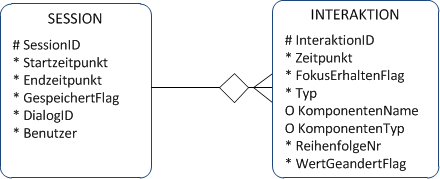
\includegraphics[]{img/ERM_UIDataCollector.PNG}
  \caption{Entity Relationship Model des UIDataCollectors nach Barker Notation \citep[vgl.][]{Inguanez2012}}
  \label{fig:ermUIDataCollector}
  \caption*{\textbf{Quelle:} eigene Darstellung}
\end{figure}
Zudem kann eine Interaktion immer nur zusammen mit einer Session aber nicht alleine exisitieren.



\subsubsection{Durchführung}

\subsection{Durchführung der Kosten-Nutzen-Analyse}
